\documentclass[conference]{IEEEtran}

\usepackage{url}
\usepackage{graphicx}

\hyphenation{op-tical net-works semi-conduc-tor}

% Document.
\begin{document}

\title{Comparative Analysis of Performance Using Server-Client Protocols}

\author{\IEEEauthorblockN{Mihail Costea, Liviu Chircu}
\IEEEauthorblockA{University Politehnica of Bucharest\\
Faculty of Automatic Control and Computer Science\\
Emails: mihail.costea90@gmail.com, liviu.chircu@gmail.com}}

\maketitle

\begin{abstract}
Current web applications' solutions for bi-directional communication are widely
based on AJAX. Even though they are well documented solutions that are backed up by
years of utilization, they have limitations imposed by the HTTP protocol. HTTP
is a stateless protocol that requires each connection to be treated as a new
connection, requiring an unnecessary overhead to communicate in both directions.
Because of these limitations, a new solution was developed - WebSockets -
which are able to natively mantain a bi-directional channel, thus reducing the
overhead imposed by connection establishment.
\\
\indent
This paper proposes to exemplify the advantages and disadvantages between
traditional HTTP implementations for bi-directional communication based on AJAX
and WebSockets. It also presents the comparison of two WebSockets
implementations, and proposes an architecture for a testing platform of
different WebSockets implementations based on the obtained results.
\end{abstract}

\IEEEpeerreviewmaketitle

% Content.
\section{Introduction}
Along with the introduction of Web 2.0, web applications have been able to
modify the content of HTML documents without the need of a complete page
refresh, offering a more interactive environment for the end-user.
The most popular technology used to create this interactivity is AJAX \cite{AJAX}
(Asynchronous JavaScript and XML). With AJAX, pages can be updated in real-time,
without needing an explicit action from the user. But because AJAX is based on
HTTP - a stateless protocol that requires each connection to be treated as a new
connection - bi-directional channels between 2 devices can only be simulated
through a series of methods which impose a significant amount of overhead, as both
nodes need to mimic this channel that require states.
Bi-directional channels are necessary for web applications such as instant
messaging clients, browser-based games, video calls, etc., where large amounts
of traffic (with complete sets of headers and message bodies) need to be sent from
each endpoint over to the opposite one.
\\

The most popular solutions used by AJAX are: \textbf{polling}, where a client sends
a request to a server at regular intervals with the server responding immediately
and closing the connection; \textbf{long-polling}, where the client requests
information from the server just as in normal polling, but the server now maintains
its connection open until it has the data to send, point in time where
it will send an immediate response;
\textbf{streaming}, where the connection between the client and the server is
kept alive indefinitely and data is streamed until one of the two closes the
connection. The problem with last solution is that AJAX
appends the new data to previously sent data until the connection ends, which is
unnecessary in many cases. Moreover, HTTP headers must be sent whenever a new
connection is created, which is a common case for polling and long-polling. If
a great amount of small pieces of data are to be sent, as in the case of a
web-based chat application, the overhead of the headers might actually overweigh
the data that is actually transmitted \cite{2009:Misc}.
\\

In order to overcome the limitations of AJAX-based solutions, the HTTP-based
WebSockets protocol was created \cite{RFC}. HTTP was chosen as a base because
most firewalls allow HTTP and HTTPS traffic  (ports 80 and 443), while other
ports' traffic might be blocked. Although based on HTTP, WebSockets do not
inherit its limitations. HTTP is only used to create and close the connection
between client and server, while the in-between information exchage is done
through a series of WebSocket-specific data frames. The distinction between
normal HTTP traffic and WebSockets is done through the "Upgrade: websocket" /
"Connection: Upgrade" headers \cite{RFC}.
\\

As mentioned above, WebSockets are a recently created technology  (the RFC was
written in 2011), so they are not supported by all major web servers, let alone
being extensively tested. This may very well be considered a downside when
compared to AJAX, which benefits from years of testing and industry usage.
Although a series of testing platforms with the purpose of validating WebSockets
implementations have been created, such as Autobahn \cite{Autobahn}, to our best
knowledge, we have yet to find any performance-oriented testing platforms for a
given WebSockets implementation.
\\

The first part of paper compares AJAX with WebSockets. It is then followed by
a comparison of two WebSockets implementations based on \textit{Node.js}.
Based on the comparison results, it proposes two different architectures for
a testing platform capable of automating the testing process.
One is independent
of the underlying Operating System and present devices. It should work for
both laptops and smartphones, for Windows and Linux and other devices and
Operating Systems. The other one is platform dependent, but it could be used
not only for testing how WebSockets behave in general, but also to assess
the behaviour of specific applications which are based on WebSockets.

\section{Related work}
Puranik et al. \cite{RT-Monitoring} exemplifies the differences in terms of
performance between AJAX and WebSockets. The authors added real-time monitoring
support for OASIS \cite{OASIS}, an open-source real-time instrumentation
middleware for distributed real-time and embedded systems. The collected
instrumentation data was sent over the Web using AJAX and WebSockets and the
results were compared. The WebSockets server consumes 50\% less network
bandwidth than the AJAX server. Also, the WebSockets client consumes memory at
a constant rate, while the AJAX client consumes it at an increasing rate.
Furthermore, the WebSockets-oriented implementation can send up to 215.44\%
more data samples than the AJAX-based counterpart although it demands the same
amount of network bandwidth.
\\

Even though WebSockets are better than AJAX based solutions, they are still
not as good as raw TCP sockets. Agarwal \cite{Performance-Penalty} discusses
the penalties of using HTML socket streams (long-polling and WebSockets) versus
TCP streams. HTML socket streams can have up to 5x protocol overhead, up to
3x more payload delivery delay and up to 3x less throughput. In case of small
data payload (a few hundreds of bytes), the performance difference between the
two becomes significantly noticeable. Also TCP streams tend to behave better
over 3G than HTML socket streams.
One reason for the poorer performance is due to the fact that the browser uses
buffering for HTML socket streams (both long-polling and WebSockets), thus 
introducing delays, while TCP sockets are able to send the data directly.
But on the good side for
WebSockets, the paper mentions that they behave better than long-polling when
it comes to sending small-sized chunks, making it a better choice for chat,
VoIP, online games, etc, just like TCP streams. A big plus for HTML sockets
over TCP streams is the fact that the data sent through them can pass over
firewalls and most proxies, as HTTP and HTTPS are commonly allowed ports.
\\

Another example where WebSockets are better than AJAX is the case of sending
small data per frame. While WebSockets exchange 2B of data per frame, continuous
polling with AJAX exchange up to 8 KB of HTTP header \cite{2009:Misc}.
\\

\section{Evaluating existing WebSocket implementations}
In order to get a better idea about how different WebSockets implementations
behave and how the architecture of the testing application should be designed, a
series of tests were performed on two different Node.js \cite{nodejs} WebSocket
implementations.
\\

The chosen implementations are \textbf{ws} \cite{nodejs-ws}
and \textbf{WebSocket-Node} \cite{nodejs-websocket}, both part of Node.js. The
tests were performed on an Intel Core i7-4770 with 16GB of RAM running on Ubuntu
13.10, 64-bit. As a measuring tool we have used the \textit{Look} performance
profiler for Node.js \cite{nodejs-look}, which offered information about the
process's CPU time, RSS (Resident Set Size), V8 heap total, V8 heap used, and
OS memory and load average. We have displayed only CPU time and RSS because we
considered them to be the most relevant, but all tests can be found at \cite{tests}.
\begin{frame}{}
  \begin{figure}
    \centering
	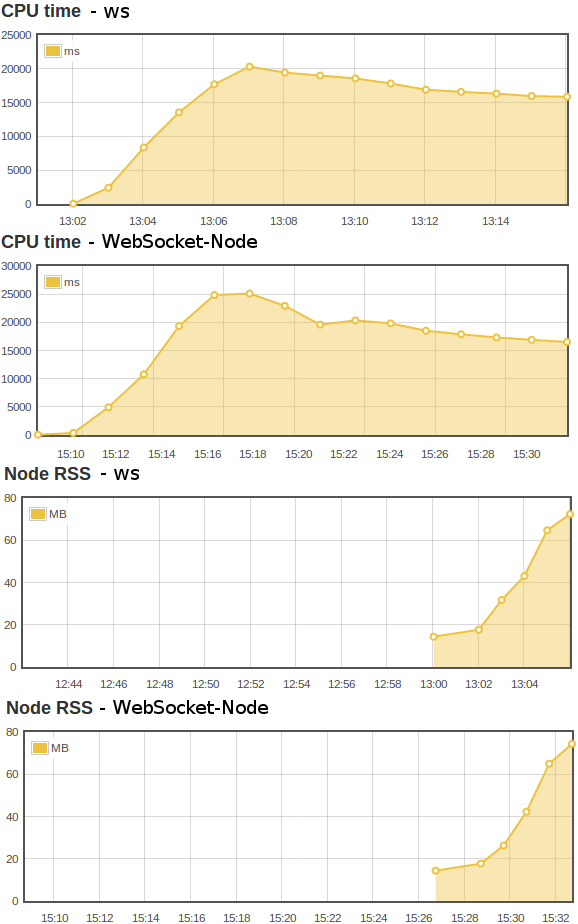
\includegraphics[width=1\linewidth]{img/test1v2.png}
    \caption{Test 1 - Constant Flow of Incoming Connections}
  \end{figure}
\end{frame}
\\

We have tested 4 different scenarios:
\\

1. Connected 4 clients simultaneously every second until 3400 connections were reached.
All connections are kept alive during the entire run and transferred data is negligible
(a single number). Figure 1 contains the comparison between the two WebSockets
implementations. We can observe that \textbf{ws} has a better CPU usage when handling
fewer connections than \textbf{WebSocket-Node}, but towards the end they behave almost
similarly. The memory consumption of the two is behaves similarly.
\\

2. Connected 600 clients simultaneously once every 120 seconds. All connections are
kept alive during the entire run and transferred data is negligible (a single number).
Figure 2 contains the comparison between the two websockets implementations.
Following the conclusions of the first example, memory consumption is similar and
\textbf{ws} is faster than \textbf{WebSocket-Node}, but under extremely heavy weight,
the system freezes faster for \textbf{ws}. We were able to go only up to 3600 connections with \textbf{ws}, while \textbf{WebSocket-Node} peaked at 4200 connections.
\begin{frame}{}
  \begin{figure}
    \centering
	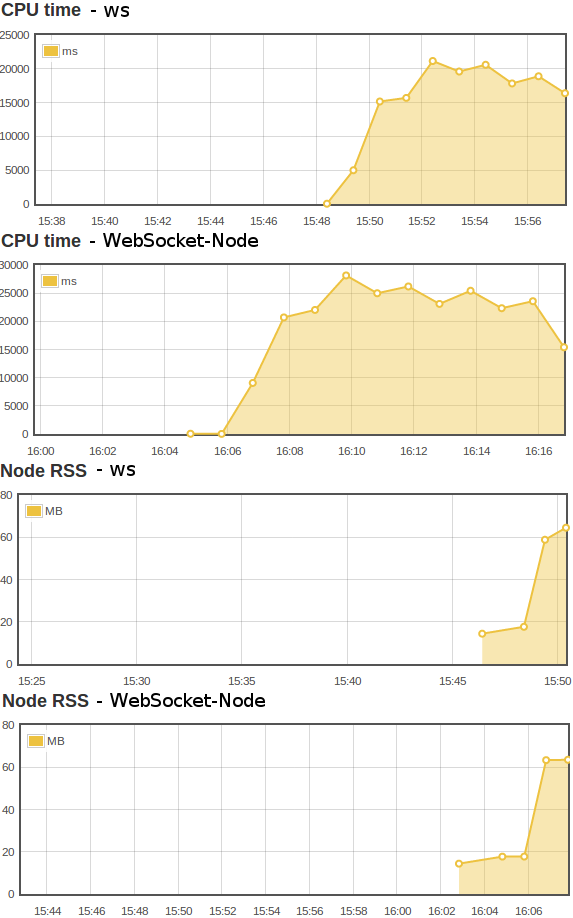
\includegraphics[width=1\linewidth]{img/test2v2.png}
    \caption{Test 2 - Bursts of Incoming Connections}
  \end{figure}
\end{frame}
\\

3. Simultaneously connected 100 clients right away, which exchanged data with
sizes ranging from 2KB up to 1MB and increments of 2KB/s per client. All
connections were kept alive during the entire run, and no extra clients were
added. Clients simply send more data with every second. Figure 3 contains
the comparison between the two WebSockets implementations. In this example
we can clearly see that \textbf{WebSocket-Node} behaves better when
sending large packets. At almost 1MB / packet, \textbf{WebSocket-Node}
processes everything in under 2s, but \textbf{ws} requires up to 6s. Also
we had to stop \textbf{ws} before 1MB / packet because the system almost
freezed, while the other implementation allowed us to let it reach its limit.
\begin{frame}{}
  \begin{figure}
    \centering
	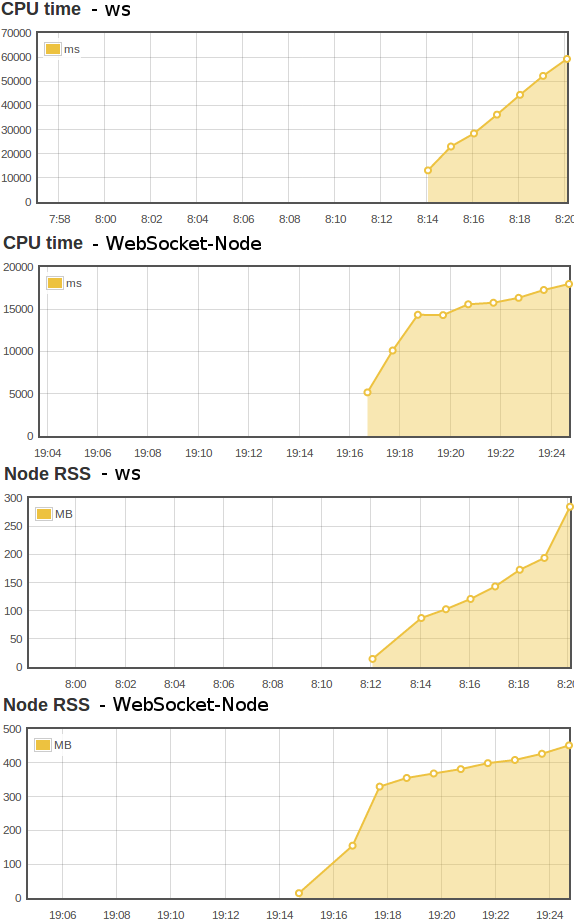
\includegraphics[width=1\linewidth]{img/test3v2.png}
    \caption{Test 3 - Constantly Increasing Volume of Data Exchanged Between a
	         Fixed Number of Clients}
  \end{figure}
\end{frame}
\\

4. Simultaneously connected 400 clients, then closed their connections after 10
seconds. Once every 90 seconds, 200 clients would be added to the prior number
of clients, and the first steps would be repeated. The process continued until 2800 connections were reached. Transferred data was negligible (a single number).
Figure 4 contains the comparison between the two websockets implementations. In
this example the used memory is similar, but the \textbf{ws} implementation has
bigger peaks for CPU usage than \textbf{WebSocket-Node} when it comes to the
last few iterations, where large numbers of connections must be managed (more
than 2200 connections). For small numbers of connections, both implementations
behave similar.
\begin{frame}{}
  \begin{figure}
    \centering
	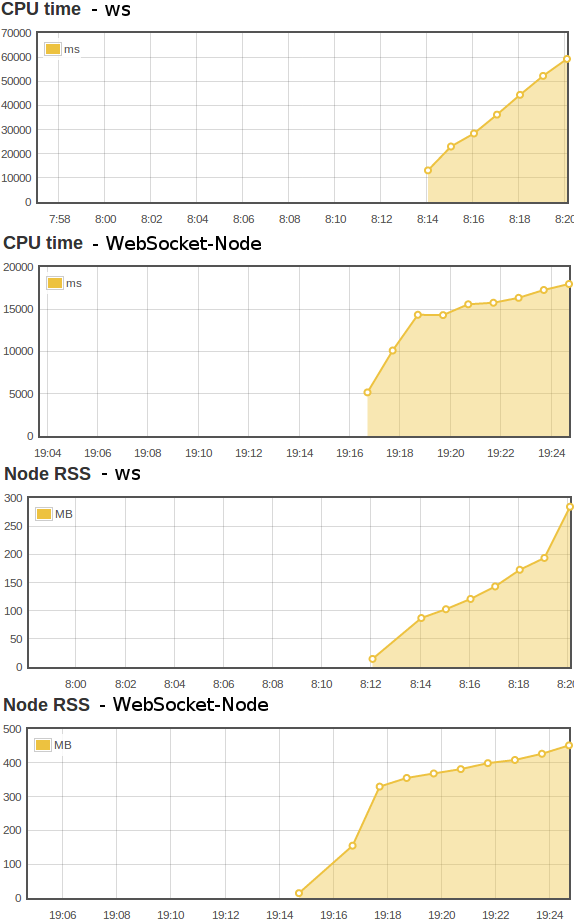
\includegraphics[width=1\linewidth]{img/test3v2.png}
    \caption{Test 4 - Linearly Increasing Number of Simultaneous Connections}
  \end{figure}
\end{frame}
\\

% FIXME: Conclusions subtitle?
We arrived at the conclusion that \textbf{ws} is faster than
\textbf{WebSocket-Node} when it comes to fewer connections and small data
packets, but with larger-sized packets and sizeable amounts of connections,
\textbf{WebSocket-Node} seems to behave better.

\section{Architecture}
This section proposes two different architectures for an application which is capable
of testing the performance of WebSockets and AJAX implementations of bi-directional
communication. The first proposal involves a generic profiling layer over
existing WebSockets implementations, coupled with the necessary modules required
in order to extract the useful data. The alternate design involves writing a
platform-dependent process analysis tool which is capable of inspecting WebSocket
proxies, together with the necessary client implementation needed in order to
perform the eventual stress tests.

\subsection{The Generic API Approach}
Figure 5 contains the architecture for the first proposal, structured into
layers. In order to test the performance automatically, the application should
be able to generate tests based on a given input and automatically measure how
these tests behave on a given platform. The design should promote easy porting
to other devices and Operating Systems. It should have a layer which is dependent
of platform and implementation. This layer is the base of a generic API that is
used by the tests generator component, the server application which communicates
directly with the tests generator, and the tracer used to gather information
about the WebSockets behavior inside the server. The API and the previously
mentioned components are going to be ported to other platforms with minimal
changes. The layer that provides the API is going to be implemented by every
platform in a different way, depending on the Operating System, specific
WebSockets API requirements, etc.
\begin{frame}{}
  \begin{figure}
    \centering
    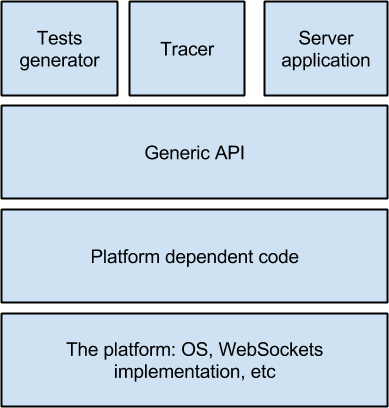
\includegraphics[width=0.45\textwidth]{img/architecture1.png}
    \caption{Testing Framework Based on a Generic API}
  \end{figure}
\end{frame}
\\

\subsection{The Platform-Dependent Alternative}
Figure 6 shows the alternate architecture. Just as before, we have a server
application and tests generator component that communicate directly. The tests
generator creates stress tests based on a user defined input, similar to Unix
commands. Similarly to the first architecture, the tracer gathers information
about the WebSockets behavior while the target server is up and running.
However, while in the first case the
tracer is a separate component that can gather information independently from
the server due to the generic API, in the current architecture the tracer is
a library used by the server directly, similar to the Look \cite{nodejs-look}
profiler. As a plus, this offers the possibility to use the tracer in other
server applications that are not created only for testing WebSockets
implementations in general, but also test the behavior of specific servers
that might be used in production and are based on WebSockets.
But this comes at the cost of portability.
For every new programming language, OS or device, the platform
dependent tool and server application need to be completely rewritten. The
tests generator does not suffer from this problem because it acts as a client
for the server and it will always make use of the same communication protocol.
\begin{frame}{}
  \begin{figure}
    \centering
    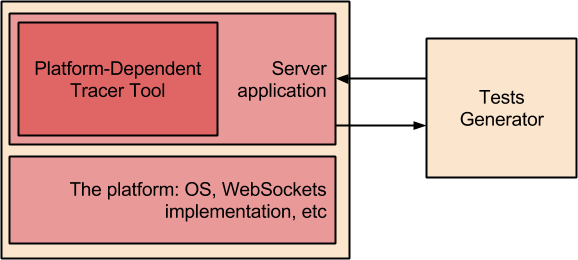
\includegraphics[width=0.5\textwidth]{img/architecture2.png}
    \caption{Testing Framework Based on a Process Monitoring Application}
  \end{figure}
\end{frame}
\\

\section{Conclusions and Future Work}
Starting with research on WebSockets and their potential in the web application
industry, we continued with a performance evaluation of a couple of existing
WebSockets implementations. Having determined the WebSockets performance caps,
we were able to propose two possibilities of designing a framework capable of
profiling existing web servers and evaluate the benefits of switching to the new 
connection-oriented WebSockets protocol. One architecture promotes easy porting
to new platforms and WebSockets implementations, with the downside that it will
initially take more time to implement and can be used only for generic testing.
The other is much more straight-forward, as its main purpose is to generate
testing results as fast as possible and maybe to be used by applications created
for production, but it comes at the cost of harder porting to other platforms.
\\

As future work, we can extend the comparative analysis to other WebSockets
implementations, such as \textbf{socket.io} \cite{socket.io}, \textbf{SockJS}
\cite{SockJS} or \textbf{Engine.IO} \cite{Engine.IO}. These comparisons might
give us better insights about which testing architecture we should choose and
how we should implement it, or maybe create a better architecture.
\\

We feel that the performance comparison framework is likely to become very popular
if properly written. Effectively seeing the benefits of switching to WebSockets
is very likely to accelerate their rate of acceptance, thus making the web an
even better, faster and more efficient place.

\bibliography{bare_conf}{}
\bibliographystyle{unsrt}

\end{document}


